% ===============================
% Data exploration
% ===============================
\newpage
\section{Accessing and exploring the Data }
\label{sec:dataaccessandexp}

As seen in the previous sections, the amount of data available in the database is enormous. In the field of computer science, the process of scanning databases for potentially interesting sets is called \textit{data mining}. What is potentially interesting completely depends on the researchers' intentions. Therefore, a multitude of filter and visualization options must be available to facilitate data exploration. Once a desired set of data has been identified, one should be able to export that data for further analysis. 

\subsection{Introducing miceminer}
\label{subsec:dataexp}

The \textit{miceminer} application intends to meet exactly these requirements. Basically, the application provides a user friendly interface to retrieve data from the database. Combined with some nifty filter capabilities and visualization options, the user gets a powerful tool to explore the data.

\textit{miceminer}'s user interface is written entirely in \textit{Flex} developed by Adobe corporation. Adobe Flex is a software development kit released by Adobe Systems for the development and deployment of cross-platform rich Internet applications based on the Adobe Flash platform \citep{wiki:flex}. The application runs within every web browser which has the \textit{Flash} plug-in version 9 or above installed. Thus, the software is cross-platform compatible, meaning that it runs on every operating system for which the \textit{Flash} player is available. 
 
Furthermore, \textit{miceminer} doesn't need to be installed on every computer, but is stored on a computer accessible over the internet, which is called a server. Every time the application is accessed, it gets downloaded to the inquiring computer, called the client. This has the comfortable consequence software updates do not need to be installed on the client's computer but instead can be deployed to the server only.     

Additionally, \textit{Flex} offers convincing tools to build interactive user interfaces and, in conjunction with third party software, dependable ways to retrieve data from a database. 

% Compared to \textit{Java}\footnote{Java is a programming language.[\ldots] Java applications can run on any Java virtual machine (JVM) regardless of the computer architecture\citep{wiki:java}.}, which has a immense \ac{API}, the one offered by \textit{Flex} is appropriate for the needs in this project.

More information about the \textit{miceminer} project, including screencasts, that illustrate features, an \ac{API} documentation, the application source code and links to other resources used for the development, can be found on the project homepage at \href{http://zool-miceminer.uzh.ch/}{http://zool-miceminer.uzh.ch}\footnote{Please note that the site is only accessible from within the network of the University of Z\"urich.}. 

\subsection{Interface}
\label{subsec:miceminer_interface}

This section gives an introduction to the user interface. User help is available on the project homepage. Furthermore, all of the components display a help button in the upper right corner of their interface. Clicking on this button reveals the help text for the component.

Figure \ref{fig:interface_overview} shows a screenshot of the \textit{miceminer} interface and identifies its main parts.

\begin{sidewaysfigure}
  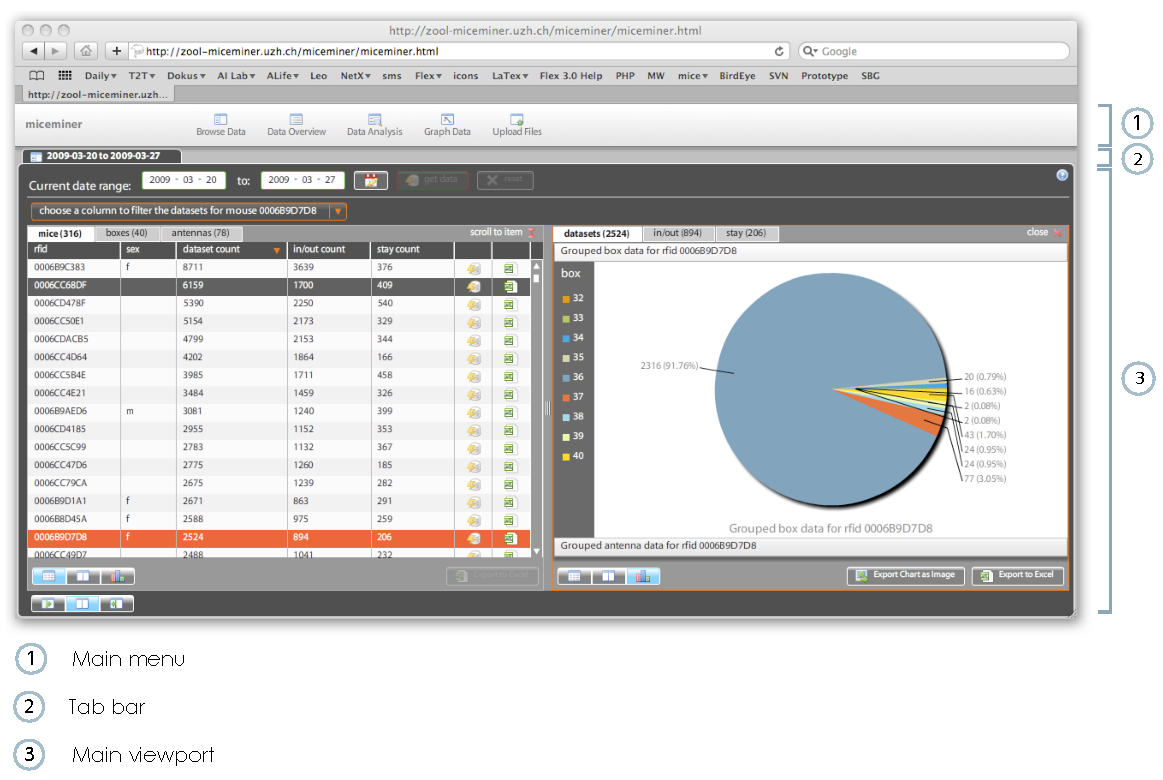
\includegraphics[width=\textwidth]{assets/pdf/interface_overview.pdf}
  \caption[\textit{miceminer} interface overview]{Screenshot of the miceminer application, displaying data for a mouse. In addition, the main parts of the interface are labeled.}
  \label{fig:interface_overview}
\end{sidewaysfigure}

From the \textit{Main menu}, the user can start the main components listed in table \ref{tab:main_components}. 

\begin{table}
\begin{center} 
\newcolumntype{H}{>{\bf}p{2.5cm}}
\renewcommand\arraystretch{1.5}% (MyValue=1.0 is for standard spacing)
\begin{tabularx}{\textwidth}{+>{\raggedleft\arraybackslash}H^X}

\toprule
Browse Data	 & This is the core component of the application and contains the functionality to explore data within a given date range. \\
Data Overview	&	Shows an overview about all the mice, (nest-) boxes, and antennas in the database. \\
Data Analysis	&	Offers some simple data analysis and evaluation methods. \\
Graph Data	 &	Interactive network representation of the data which shows possible social relationships within the mice community. \\
Upload Files	&	Components to perform administrative tasks. This component is password protected and is only used by the system administrators. \\\bottomrule
\end{tabularx}
\captionof{table}[\textit{miceminer} main menu]{Main components selectable from the \textit{Main menu} of the \textit{miceminer} application.}
\label{tab:main_components}
\end{center}
\end{table}

A main component is started by clicking on an icon in the \textit{Main menu}. This will result in its interface being shown in the \textit{Main Viewport}. Furthermore, a tab is added to the \textit{Tab Bar}. The \textit{Tab Bar} allows the user to switch between the open components by clicking on the appropriate tab.

The interface arrangement is the same in all components except for the \textbf{Graph Data} component. Figure \ref{fig:interface_component} identifies the different parts by means of a screenshot of the \textbf{Browse Data} component.

\begin{figure}[!htbp]
\begin{center}
  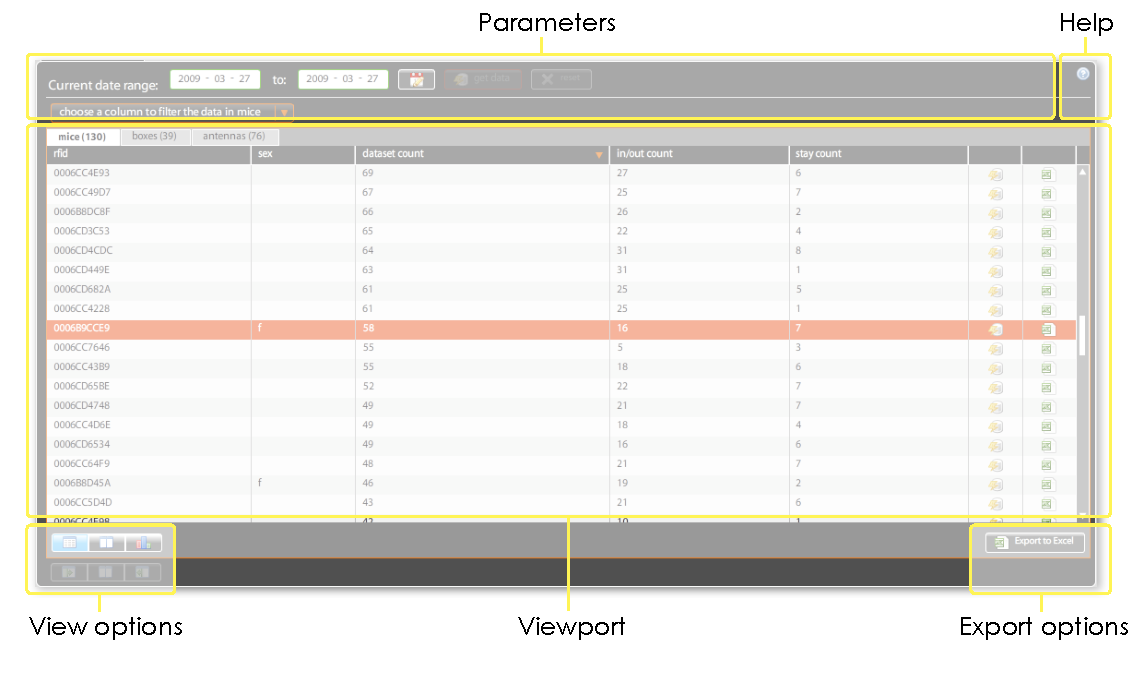
\includegraphics[width=\textwidth]{assets/pdf/interface_component.pdf}
  \caption[\textit{Browse Data} component interface]{Screenshot of the \textbf{Browse Data} component, with labeled parts of the interface.}
  \label{fig:interface_component}
\end{center}
\end{figure}

In the \textit{Parameters} section, the user sets the factors influencing data displayed in the \textit{Viewport}. When the \textit{Help} button is clicked, a window will pop up containing instructions to use the actual component. An \textit{Export option} to save the tabular data as an \textit{Excel} worksheet is available in every component. Some components offer additional export formats, depending on their function. The \textit{View options} (pictured in detail in figure \ref{fig:view_options}) are used to switch between tabular (see section \ref{sububsec:datafilter}) and chart view (see section \ref{subsubsec:datavis}). \textit{View options} are only available in the \textbf{Browse Data} component.

\begin{figure}[htpb]
\begin{center}
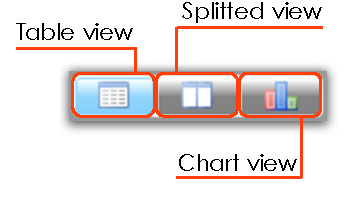
\includegraphics[width=.3\textwidth]{assets/pdf/view_options.pdf}
\caption[View options]{The \textit{View Options} for the \textbf{Browse Data} component. The split view is selected to get table and chart views side by side.}
\label{fig:view_options}
\end{center}
\end{figure}    

\subsection{Software design}
\label{subsec:miceminer_design}   

\textit{Flex} itself does not include methods to query a database. Instead, the application sends its requests to a \textit{PHP}\footnote{PHP is a scripting language originally designed for producing dynamic web pages\citep{wiki:php}.} file stored on the server, thereby providing the necessary methods. These methods handle the database queries and send the results back to the \textit{Flex}-based \textit{miceminer} application running on the client computer. An auxiliary software (\textit{amfphp}\footnote{Visit \href{http://www.amfphp.org}{http://www.amfphp.org} for details.}) speeds up the data transfer between the server and the client.

\textit{PHP} provides ways to export data to different file formats such as \textit{Excel}. Additional export options have been designed so data can be analyzed by other scientific softwares.

The way user interface software components interact is illustrated in figure \ref{fig:app_design_miceminer}. Readers interested in the actual programming should refer to the \textit{Additional Sites}\footnote{\href{http://zool-miceminer.uzh.ch/\#additional_sites}{http://zool-miceminer.uzh.ch/\#additional\_sites}} section on the project~homepage.   

\begin{figure}[htpb]
\begin{center}
  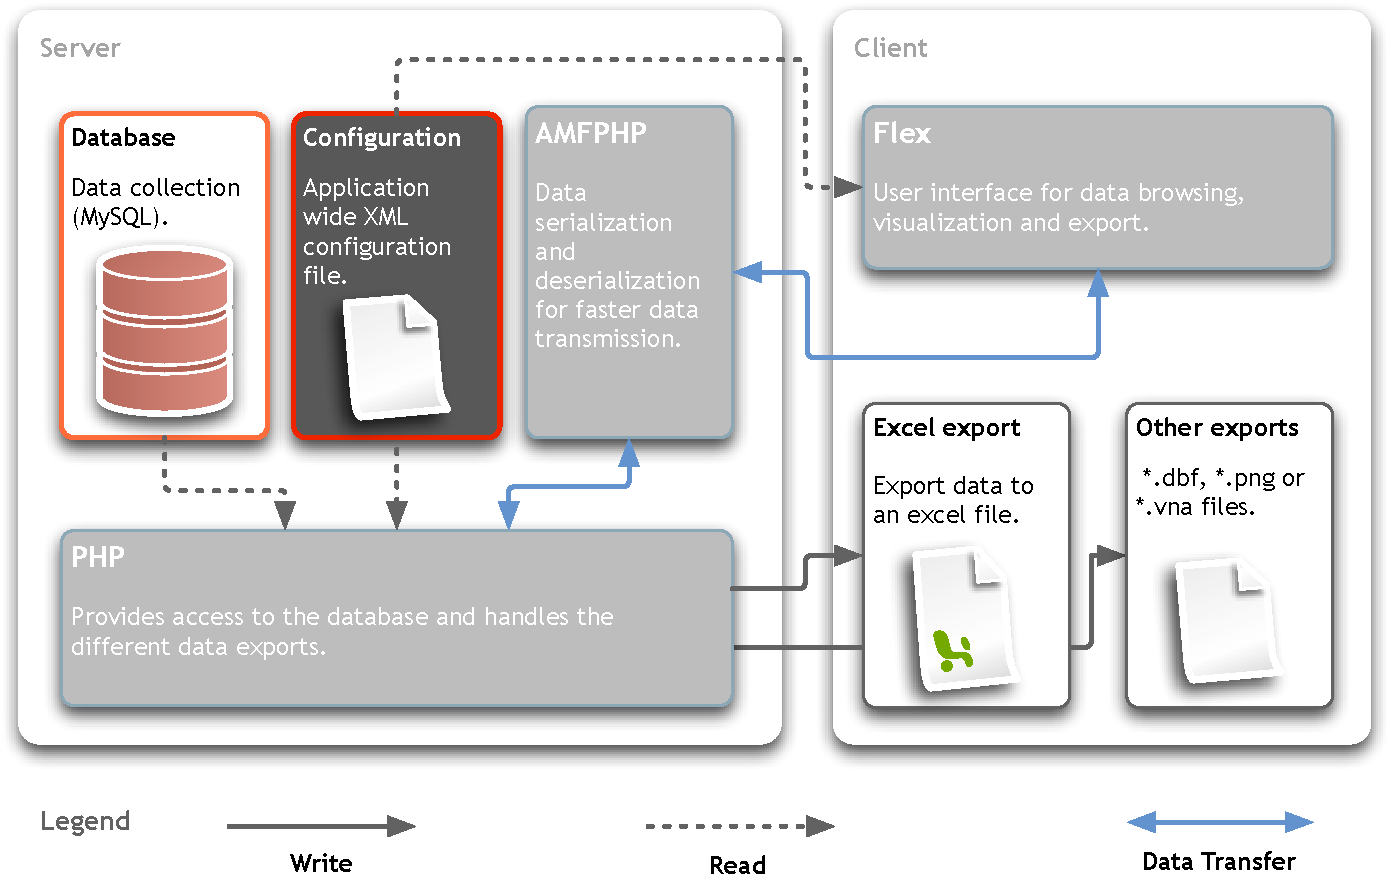
\includegraphics[width=\textwidth]{assets/pdf/application_design_miceminer.pdf}
  \caption[Schema of the user interface design]{Schema of the user interface design.}
  \label{fig:app_design_miceminer}
\end{center}
\end{figure}

\subsection{Configuration}
\label{subsec:miceminer_config}

As pictured in Figure \ref{fig:app_design_miceminer}, the relevant parts read their configuration from the same XML file as the data processing scripts. 

A detailed explanation of the part of the configuration file where the user interface can be configured is beyond the scope of this document. The influence of the different values is explained within the file. As an example, the configuration of the main components is shown in Appendix \ref{lst:comp_config} on page \pageref{lst:comp_config}.

The most important parameter, which can be changed easily, is the \lstinline|<maxStay>| value. This value sets the upper limit of a \textit{stay} or a \textit{meeting result} in hours, to be included in the displayed data. It had to be introduced due to the impractical duration of stay values in the \textit{stay results} (see section \ref{subsec:stayres} and \ref{subsec:meetingres} for details).

\subsection{Basic application concept and implementation}
\label{subsec:app_concept}

On the one hand, the software intends to offer a variety of ways and means to browse the data, while on the other hand, ease of use should be assured. Software design and user interface were refined through frequent feedback from researchers. This section details the application's three main functionalities.
   
\subsubsection{Data filtering}
\label{sububsec:datafilter}

The database includes several different types of data (antenna readings, \textit{direction results}, \textit{stay results} and \textit{meeting results}) which can be allocated to the different system members (mice, boxes, and antennas). There are therefore various approaches to explore data. One researcher, for instance, could be interested in readings for a mouse at a given antenna, another one needs to know in which boxes a specific mouse has spent time. What both approaches have in common is that the data is usually analyzed over a specific period. Hence, the period is defined to be the starting point for every session (see figure \ref{fig:date_period}).

\begin{figure}[htpb]
\begin{center}
  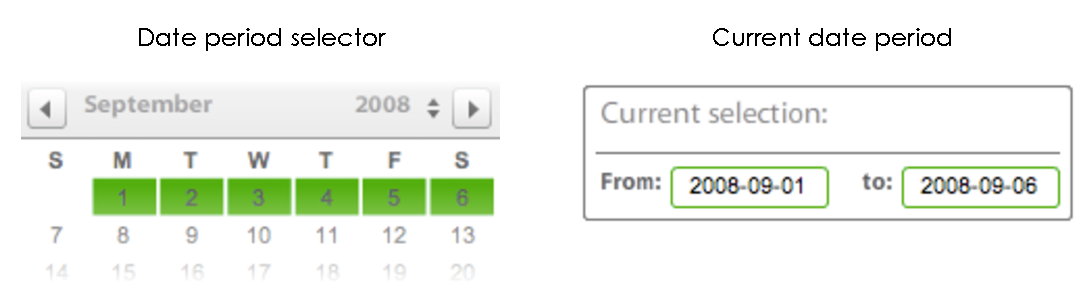
\includegraphics[width=.75\textwidth]{assets/pdf/date_period.pdf}
  \caption[Date period selector]{Date period selector and current selection.}
  \label{fig:date_period}
\end{center}
\end{figure}

The user is then provided with three tables listing mice, boxes, and antennas, respectively, for which data in the selected period could be found. For each table element the exact counts of antenna recordings, \textit{direction results}, \textit{stay results} and some additional information about the item is displayed alongside (see figure \ref{fig:data_overview_with_count}). These tables therefore present a data summary that can serve as a basis for the selection of interesting items. 

\begin{figure}[htpb]
\begin{center}
  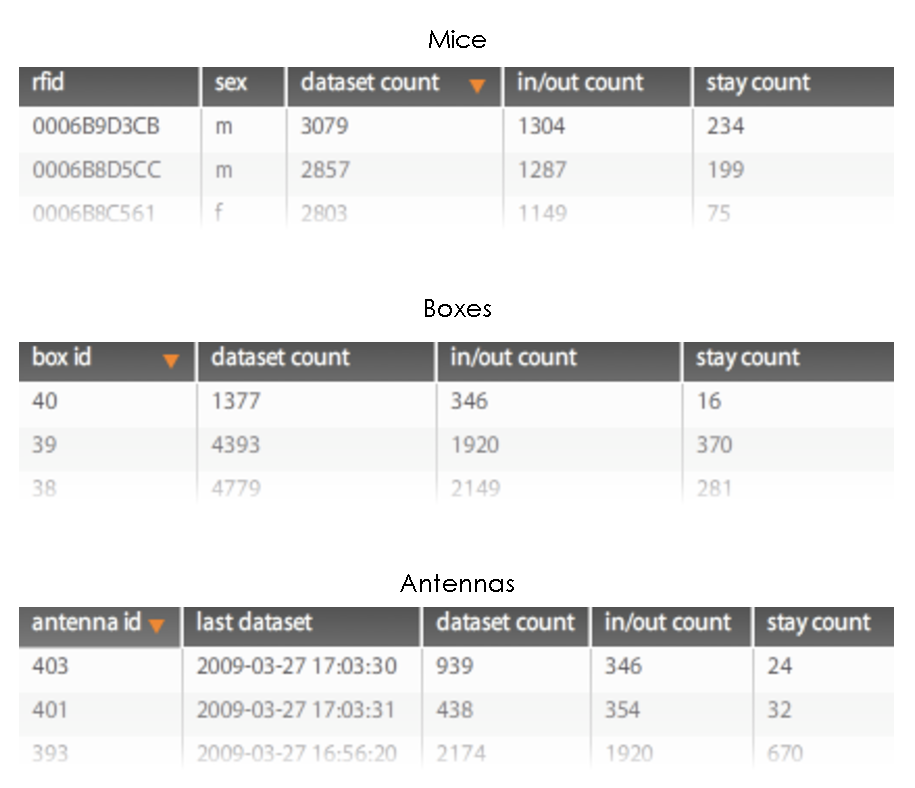
\includegraphics[width=.66\textwidth]{assets/pdf/overview_list.pdf}
  \caption[Overview of the summarized data for mice, boxes and antennas within a date period]{Overview of the mice, boxes and antennas with the respective counts for a selected period. The number of \textit{direction results} are labeled \textbf{in/out count}, the \textit{stay results}  \textbf{stay count}.}
  \label{fig:data_overview_with_count}
\end{center}
\end{figure}

With a click on the column header, the data gets sorted ascending or descending. Moreover, the data displayed in the tables can be constrained by setting filters. For each column a filter can be chosen from a central drop down menu. The menu content follows user focus, meaning that if the user switches to another table, the filter menu is updated to reflect the available filters for the selected table. The type of filter depends on the kind of data the column contains. For a column containing text values, for instance, the appropriate filter is a text box where the user can type in the text to search for. Figure \ref{fig:filter_types} shows an overview of the filter types.

\begin{figure}[ht]
\begin{center}
  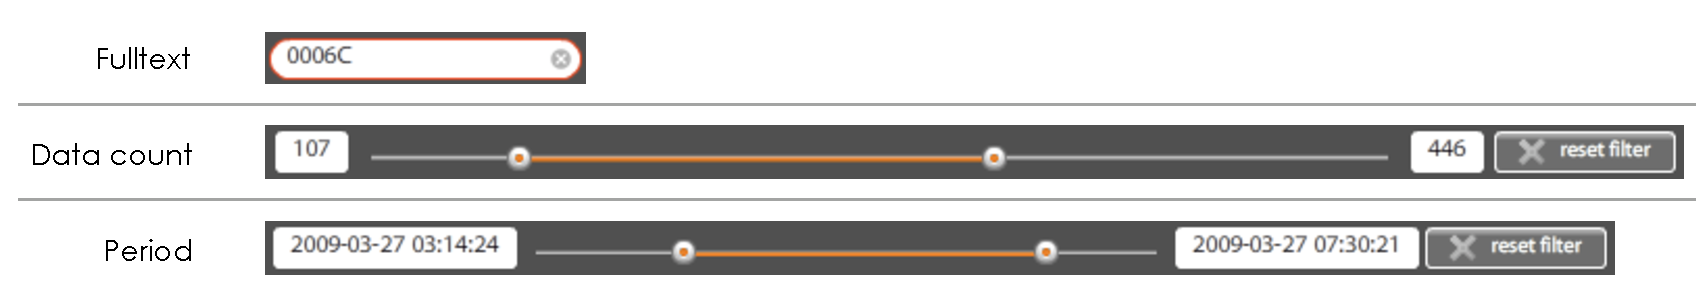
\includegraphics[width=\textwidth]{assets/pdf/filter_types.pdf}
  \caption[Filter types]{The \textit{Fulltext} filter searches the column data for the typed text. The \textit{data count} and \textit{Period} filters allow to set a lower and an upper limit by using the two sliders.}
  \label{fig:filter_types}
\end{center}
\end{figure}

Based on the tables with summarized data, the user can choose the mouse, box, or antenna for which to obtain detailed data. Two data retrieval options are available: the first one displays the data in the application, the second one exports the data directly to an \textit{Excel} worksheet (see figure \ref{fig:get_data_options}). The latter option has been added as it allows the user to quickly download the data and analyze it in another tool. Also, the \textit{miceminer} application fails to display more than approximately 20,000 rows of data. Export to \textit{Excel} overcomes this limitation.   

\begin{figure}[htbp]
\begin{center}
  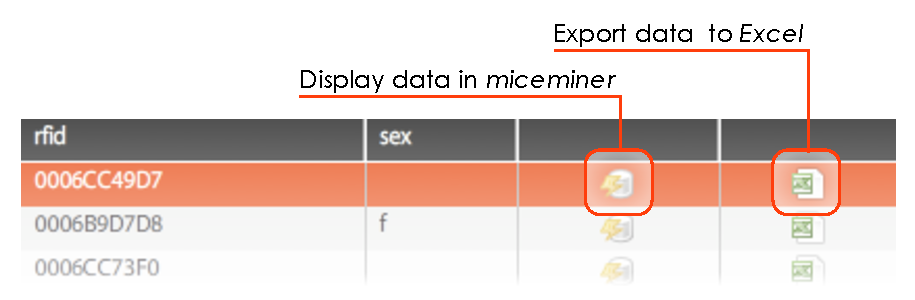
\includegraphics[width=.75\textwidth]{assets/pdf/get_data_options.pdf}
  \caption[Data retrieval options]{Data retrieval options.}
  \label{fig:get_data_options}
\end{center}
\end{figure}

If the user chooses to show the data in the application, a secondary group of tables containing the antenna recordings, \textit{direction results} and \textit{stay results} is shown in the right part of the \textit{Viewport} (see figure \ref{fig:overview_data} for clippings of the tables containing the data for a mouse). The column-based filters work exactly the same as in the tables with the summarized data to ensure usability and avoid interface clutter. 

\begin{figure}[htpb]
\begin{center}
  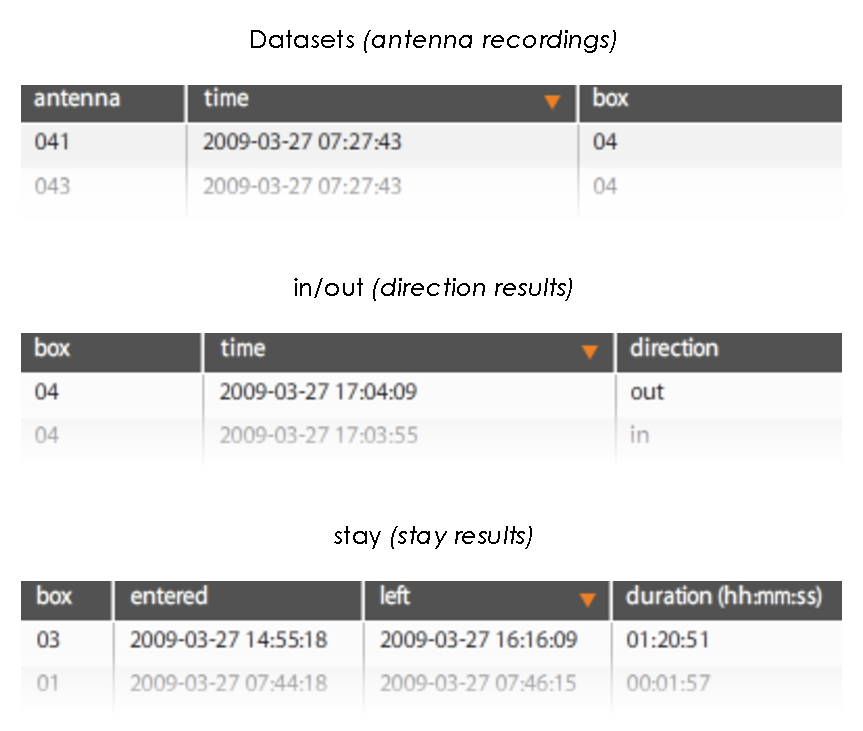
\includegraphics[width=.66\textwidth]{assets/pdf/overview_data.pdf}
  \caption[Clippings of the tables containing the results for a mouse]{Clippings of the tables containing the antenna recordings, \textit{direction results} and \textit{stay results} for a mouse.}
  \label{fig:overview_data}
\end{center}
\end{figure}  

With the whole package of filter options, starting with the period and ending with the column based filters, the user is able to explore and export the data at every level.       

\subsubsection{Data visualization}
\label{subsubsec:datavis}

Sometimes it might not be convenient to look at tables to get an idea of how an item, a mouse for instance, is positioned by its numbers in comparison to the others. Furthermore, distributions are better illustrated by the use of a pie chart. 

For the visualization of the tables containing the summarized data, the chart view displays a column chart. The x-axis values are either the mice, the boxes, or the antennas with their respective counts of antenna recordings (data count), \textit{direction results} (in/out count), and \textit{stay results} (stay count) as the y-axis values (see figure \ref{fig:mouse_chart_item} for an example of a chart item for a mouse). If the chart is visible, an option to export the chart as an image is available.

\begin{figure}[!htbp]
\begin{center}
  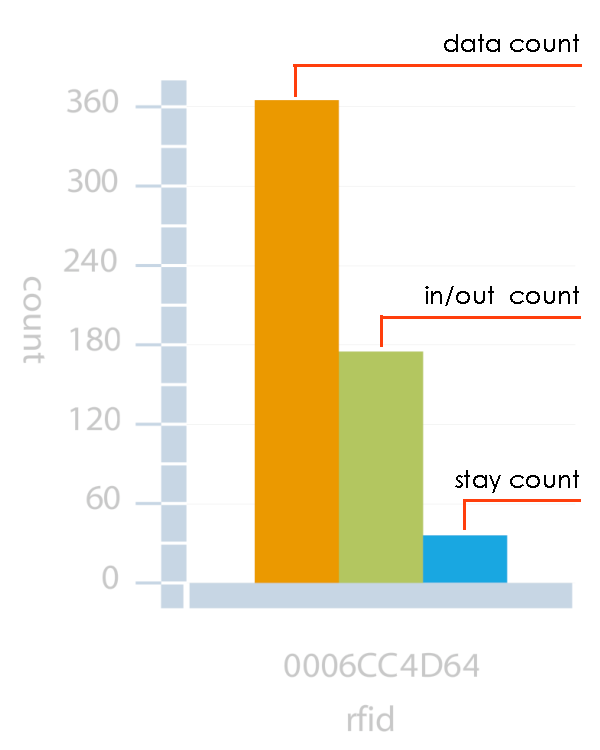
\includegraphics[width=.33\textwidth]{assets/pdf/mouse_chart_item.pdf}
  \caption[Chart item for a mouse with corresponding data counts]{Chart item for a mouse with corresponding data counts.}
  \label{fig:mouse_chart_item}
\end{center}
\end{figure}

As in the table view, the chart view offers the same sorting, filter, and export options. Furthermore, if a sort or filter has been applied in one of the views, or another item is selected, this change is updated in the other view. This is best seen if the split view is selected, as shown in figure \ref{fig:table_chart_view}, to have the table and the chart view side by side. Thus, the user is able to quickly find a mouse, box or antenna, which might be of special interest for further analysis.

\begin{figure}[htpb]
\begin{center}
  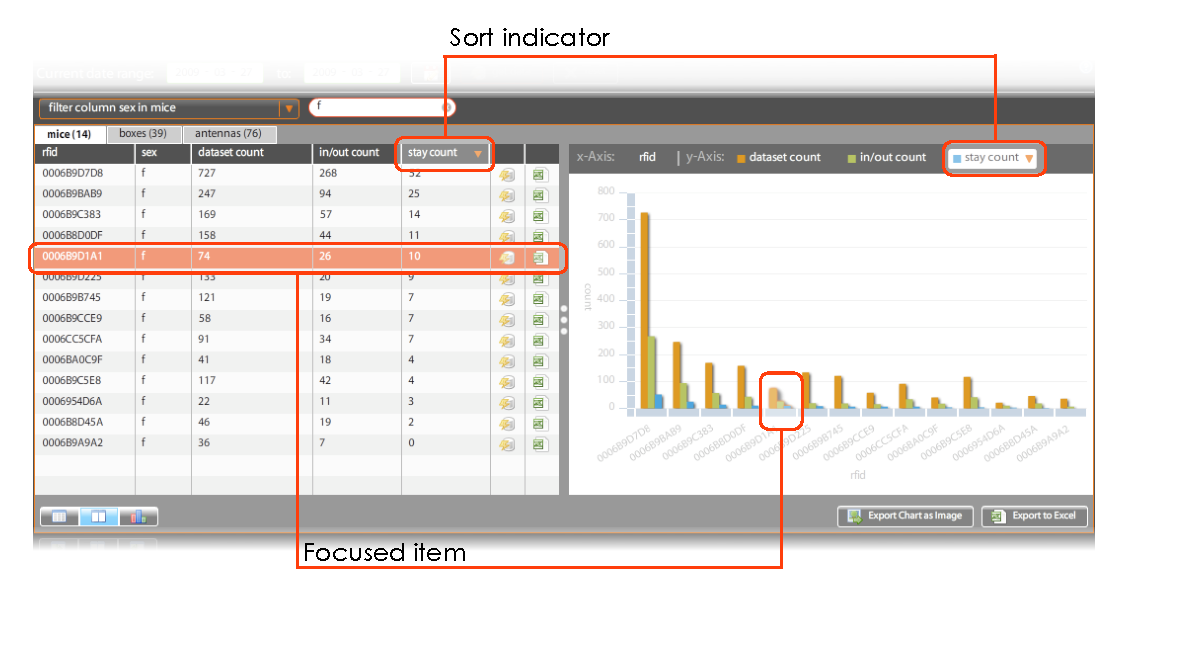
\includegraphics[width=\textwidth]{assets/pdf/table_chart_view.pdf}
  \caption[Split view]{Split view in in the \textbf{Browse Data} component. Indicated are the values which are synchronized in both, the table and the chart view.}
  \label{fig:table_chart_view}
\end{center}
\end{figure}

The chart view for the actual results of a mouse, box, or antenna is different, because the researchers are usually interested in the distribution of the results. Therefore, the data is grouped on values in a column and displayed as a pie chart (see figure \ref{fig:pie_chart_for_mouse}). Accordingly, \textit{Excel} export behavior changes as well. Other than in the tabular view, not the list, but the grouped data underlying the chart is exported.

\begin{figure}[htbp]
\begin{center}
  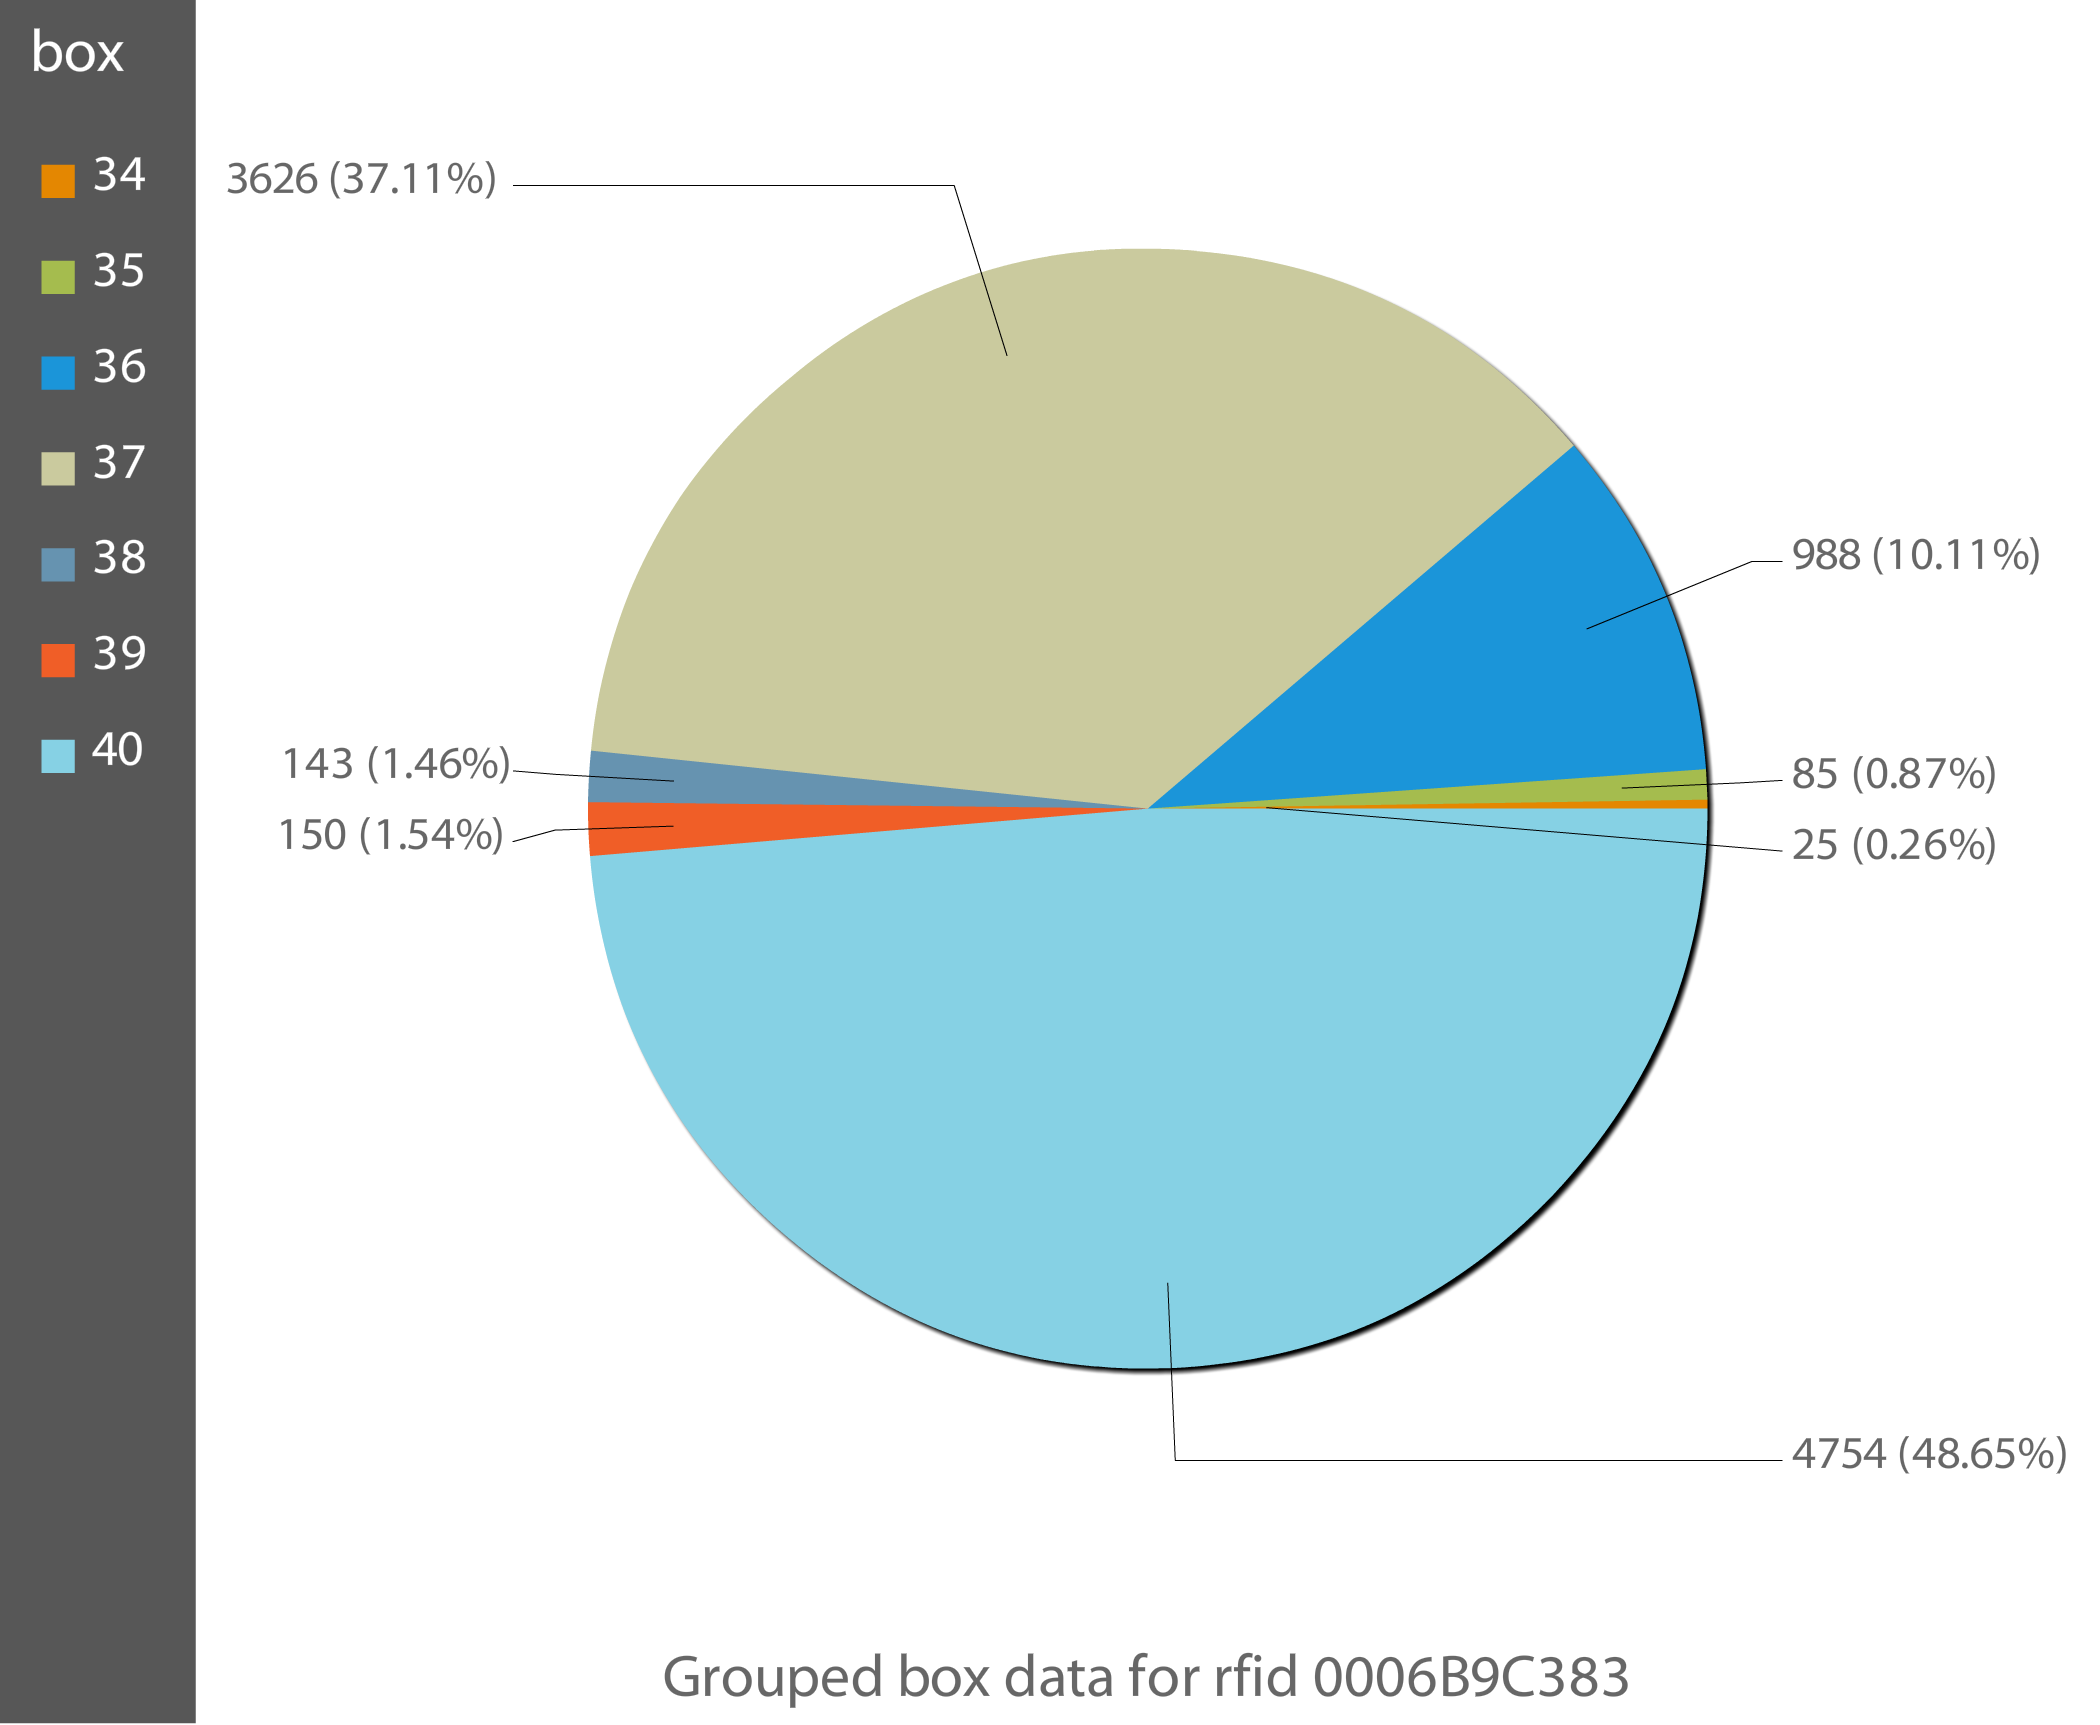
\includegraphics[width=.66\textwidth]{assets/img/pie_chart_for_mouse.png}
  \caption[Pie chart of result data for a mouse]{Pie chart with grouped box recordings for a mouse. The chart shows how many times the mouse has been recorded at the antennas of the boxes listed in the legend on the left side (e.g. 4754 times at box 40) during the selected period.}
  \label{fig:pie_chart_for_mouse}
\end{center}
\end{figure}

In addition, a secondary chart can be accessed. If the user double-clicks a pie chart item, for example the one for box 40 in figure \ref{fig:pie_chart_for_mouse}, another pie chart will be displayed alongside. In this case, the secondary chart shows which other mice have been recorded at box 40 during the selected period. In fact, this secondary chart is the same as if the user selects the chart view of the results for box 40 in the same period. Hence, the secondary chart is more of a handy method to view both information at the same time.

Combined with the shared filter capabilities and the export options, the visualization offers a good alternative to explore the data. A special visualization, which shows possible positive social relationships between the mice living in the barn is presented in section \ref{sec:graph}.

% ----------------------------------------------
% Data analysis
% ----------------------------------------------
\subsection{Simple data analysis with miceminer}
\label{subsec:data_ana} 

The \textit{miceminer} application provides some simple data analysis functionality based on the ideas from researchers involved in the project.

\subsubsection{Home range}
\label{subsubsec:homerangedata}

To carry out home range analysis, the positions of the nestboxes within the barn have been added to the database. The interface consists of a selector to choose the rfid and another one for the period, the data should be retrieved for\footnote{The data used in this component originates from the \lstinline|data| table (see section \ref{para:data_table} on page \pageref{para:data_table}).}. Once these values are set, the user can decide if the data should be exported into a \textit{dBase} (file extension .dbf) file, or if a calculation of the \textit{Minimum Convex Polygon (MCP)} should be executed. Figure \ref{fig:home_range} shows a labeled screenshot of the component interface.

\begin{figure}[htpb]
\begin{center}
  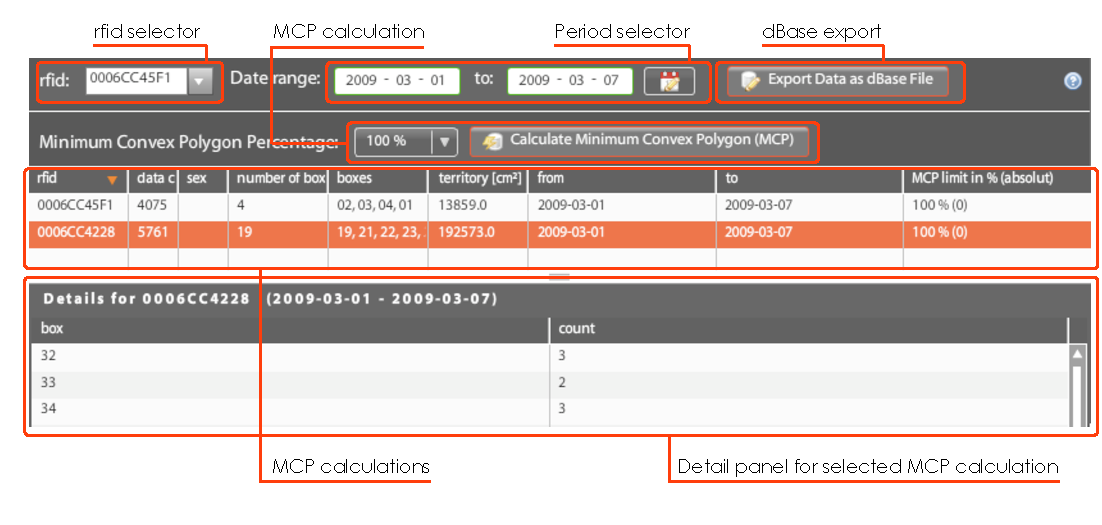
\includegraphics[width=.75\textwidth]{assets/pdf/home_range.pdf}
  \caption[\textit{Home range} component interface overview]{Interface of the component to retrieve data for a subsequent home range analysis or to calculate an MCP.}
  \label{fig:home_range}
\end{center}
\end{figure}

The exported \textit{dBase} file includes all the information needed for a home range analyses using \textit{ArcGIS}\footnote{Visit \href{http://www.esri.com/software/arcgis/}{http://www.esri.com/software/arcgis/} for details about \textit{ArcGIS}.}, a software widely used for spatial analysis. 

If the selected mouse has been recorded at more than two nestboxes during the selected period, we get a polygon spanned by the position of these nestboxes. This area can be calculated, and is called the minumum convex polygon (MCP). Figure \ref{fig:mcp} shows an example for an MCP calculated for a mouse that visited nestboxes 12 to 17. 

\begin{figure}[htpb]
\begin{center}
  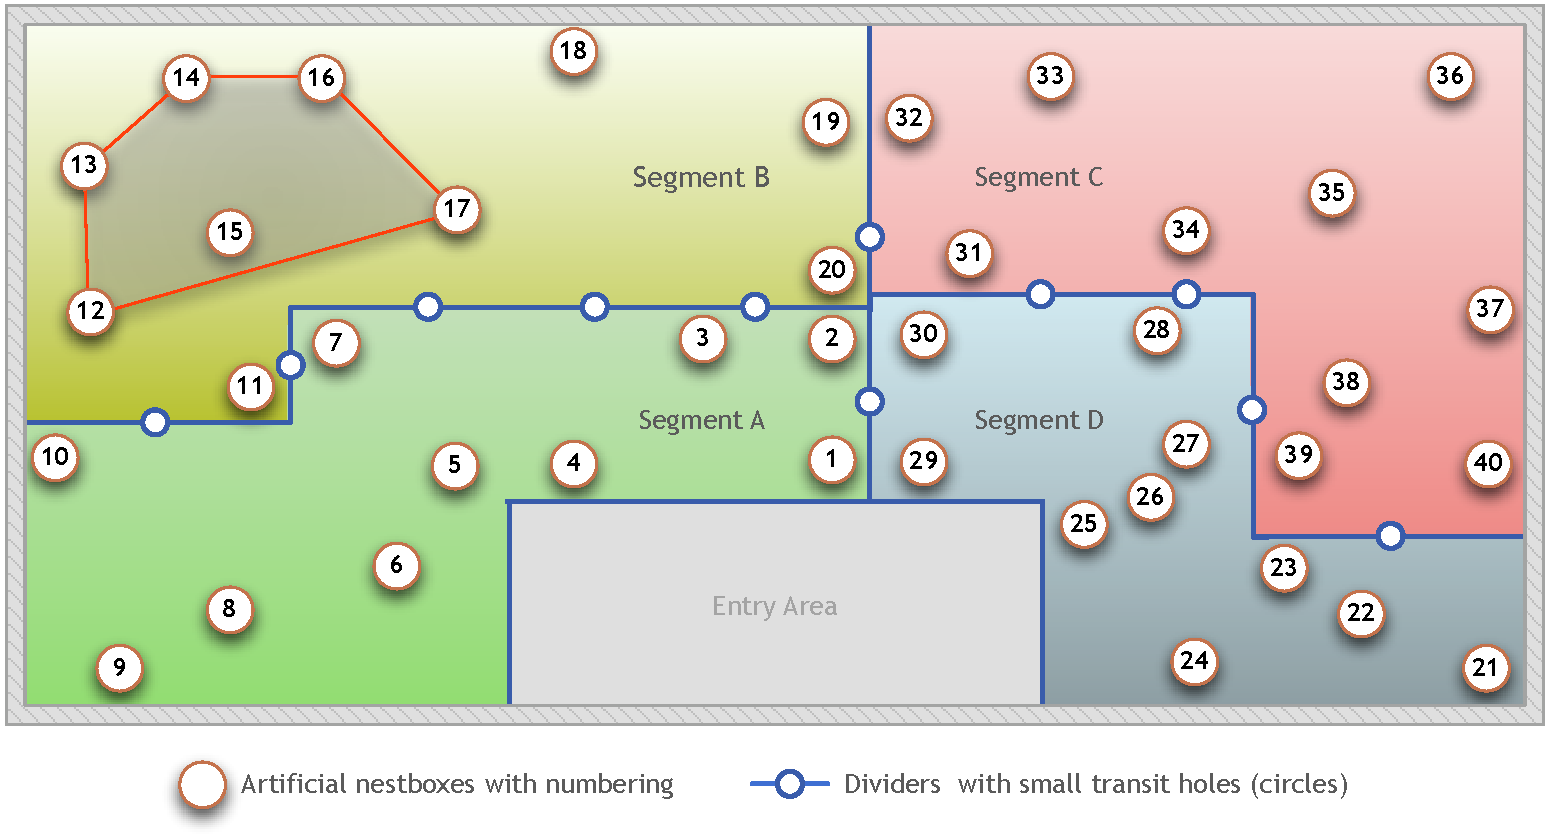
\includegraphics[width=.75\textwidth]{assets/pdf/mcp.pdf}
  \caption[Minimum convex polygon (MCP)]{An MCP for a mouse which visited nestboxes 12 to 17. In addition, the coordinate system is indicated.}
  \label{fig:mcp}
\end{center}
\end{figure}

 % sensitive <> sensible, check dictionnary -tnetter 11/09/2009 14:56
 % Actually the same in german. But in german, the distinction is not made that clear. However, in this context, sensitive is truly better. 
Since this method of determining the home range is very sensitive to outliers, the MCP can be limited to the nestboxes with an adequate number of datasets. This is accomplished by selecting an appropriate percentage value for the MCP calculation. If the value is set to 100\%, all the nestboxes, independent of their data count, are included in the calculation. For a value of 90\%, the nestbox must have a data count which is equal or greater than 10\% of the sum of the data count for all the nestboxes. The following example which is based on the situation shown in figure \ref{fig:mcp} should clarify the method.

\begin{table} 
\begin{center} 
\newcolumntype{H}{>{}p{2cm}}
\renewcommand\arraystretch{1.2}% (MyValue=1.0 is for standard spacing)
\begin{tabularx}{.4\textwidth}{+>{\raggedright\arraybackslash}H^X}
\rowstyle{\bfseries}
Nestbox	& Data count \\\midrule
12	&	44 \\
13	&	62 \\
14	&	80 \\
15	&	52 \\
16	&	12 \\
17	&	4 \\
\midrule
\rowstyle{\bfseries}
Sum	&	254
\end{tabularx}
\captionof{table}[Sample distribution of data counts to the nestboxes]{Representative distribution of the data counts for the nestboxes 12 to 17.}
\label{tab:mcp_example}
\end{center}
\end{table}
% example <> exemplary, this is quite subtle, check dictionnary -tnetter 11/09/2009 14:58
% In the dictionary it sais:  exemplary -> serving as an example, instance, or illustration. I don't see what was the problem here. Maybe to subtle for me.

With the threshold set to 90\%, a nestbox must have at least a data count of $25.4$ (10\% of 254). Nestboxes 16 and 17 are below this value and will be excluded from the calculation. Considering figure \ref{fig:mcp}, one can see how the MCP, and therefore the home range, diminishes strikingly due to this limitation. 

The data count distribution is shown in the detail panel of the interface (labeled in figure \ref{fig:home_range}), to simplify the selection of the right percentage value.     

\subsubsection{Shared preferences}
\label{subsubsec:sharedpref}

The component is used to figure out if two female mice spent more time together in a nestbox as expected. This is the case if two mice have some kind of a positive social relationship, for example caused by relatedness.

Figure \ref{fig:shared_pref} shows the component interface consisting of two controls to select the female mice and a chooser for the period. The nestbox selector allows the user to restrict the calculation to a specifc nestbox.

\begin{figure}[htpb]
\begin{center}
  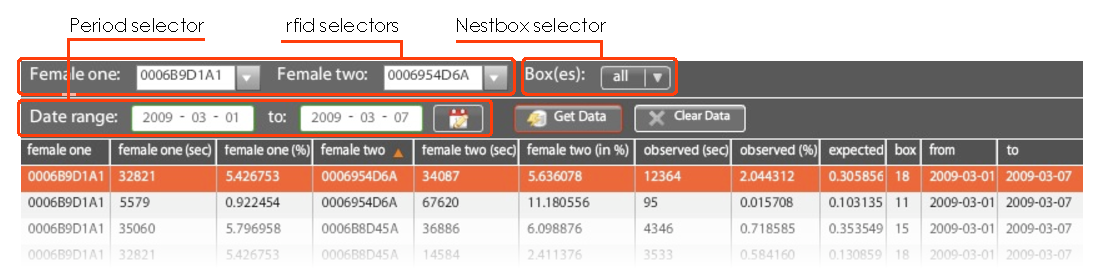
\includegraphics[width=\textwidth]{assets/pdf/shared_pref.pdf}
  \caption[\textit{Shared preferences} component interface overview]{Interface overview of the \textit{Shared preferences} component.}
  \label{fig:shared_pref}
\end{center}
\end{figure}

The calculation starts by retrieving the time each of the two mice spent in a nestbox from the \lstinline|result| table (see section \ref{para:res_table} on page \pageref{para:res_table}). These time values are put into relation to the time the two mice spent together in a nestbox, which can be determined by querying the \lstinline|meetings| table (see section \ref{para:meetings_table}). Resulting are relative values for the expected and the observed time which can be compared. 

\subsubsection{Monthly box \& monthly antennas}
\label{subsubsec:monthbox}

Both components have been created to support Olivia Dieser in her work to determine the territorial behavior of mice (see section \ref{subsec:results}).

The user selects a month, and optionally a period of the time of day, and obtains a table where columns denote the nestboxes and each row represents a mouse (see figure \ref{fig:month_box_ant} for a screenshot with labeled controls). The respective data counts are found in the intersection of the nestbox (column) and the mouse (row).

In the case of the \textbf{Monthly Box} component, the \lstinline|direction results| with a direction value of \lstinline|in| (see section \ref{para:dir_table} on page \pageref{para:dir_table}) are searched for the appropriate data. For the \textbf{Monthly Antenna} component, the data is retrieved from the \lstinline|data| table (see section \ref{para:data_table} on page \pageref{para:data_table}).

\begin{figure}[htpb]
\begin{center}
  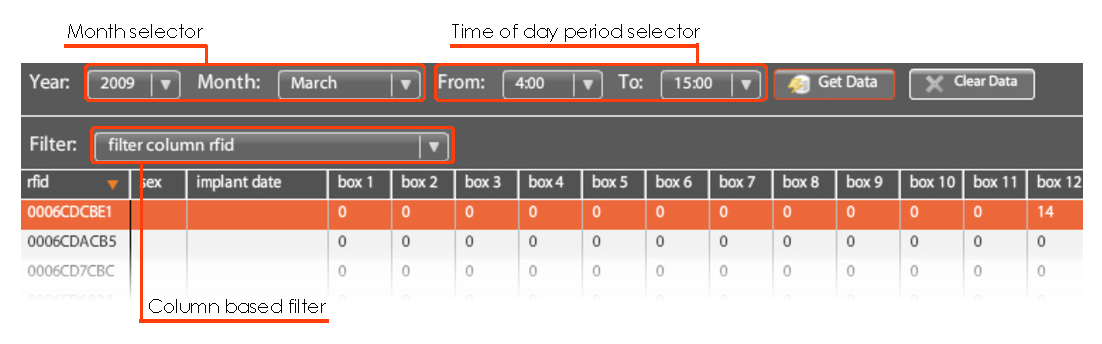
\includegraphics[width=\textwidth]{assets/pdf/month_box_ant.pdf}
  \caption[\textit{Monthly box} component interface overview]{Interface overview of the \textit{Monthly box} component.}
  \label{fig:month_box_ant}
\end{center}
\end{figure}

The option to select a period of the time of day is used to perform a differentiated analysis of the territorial behavior of the mice during phases of higher and lower activity.

\subsection{Results}
\label{subsec:results}
 
Although there is ongoing or planned research using the different functionalities the \textit{miceminer} application offers, not much results are available yet. Mainly because the genetical analysis of the mice is not complete. 
 
In conjunction with the genetic data, the \textit{miceminer} application allows for several types of analysis. For instance by using the spatial position data to identify possible kin structures in the barn or the nestboxes, or the shared preferences analyses (see \ref{subsubsec:sharedpref}) to determine preferential social attachment. 
 
However, one result can already be presented.
 
Olivia Dieser \citep{dieser:08} carried out a long-term analysis to investigate the territorial social behavior of the house mice population living in the barn (see section \ref{sec:shedsetup}). Data used in this work has been retrieved via the \textit{miceminer} application (see section \ref{subsubsec:monthbox}). Based on the data of 321 individual mice, collected over a period of 15 months, the influence of gender, season and time of day, on the usage of the nestboxes was analyzed. Furthermore, the seasonal influence on the composition of the mouse population has been determined. Refer to section \ref{subsec:collectspatialpos} for details about the artificial nestboxes and the system which is collecting the data.
 
During summer, when the mating activity is high, more female than male mice lived in the barn, while in winter the ratio was about one. This result can be explained by the polygynandric mating behavior of the house mice. Only dominant male mice get access to a female for mating. Hence, subdominant male mice may be banished from the barn by the dominant mice. This hypothesis is supported by the finding that overlap of male terretories is less in summer than in winter. 
 
Females, on the other hand, used more boxes during the summer, possibly to increase their chances of mating with many different males or to improve access to resources for weaned offspring.
 
In general, female mice visited more different artificial nestboxes than male mice. This could be explained by the limit of boxes male mice can defend to mark their territory.